\chapter{Conclusions}


\section{Summary of Contributions}

In this thesis we have presented our contributions to different components of an ambisonics analysis and generation framework, with a focus on reproducibility and portability to real-world scenarios.
The main scientific objectives of this thesis, as they were described in Section \ref{sec:objectives}, are: 
 

\begin{enumerate}
	\item The development of methods to support and improve the characterization of acoustic parameters.
	\item The research on parametric-based methodologies for sound event localization and detection.
	\item The contribution in the generation and storage of annotated ambisonic datasets.
\end{enumerate}

In what follows, we summarize the main contributions of the present thesis, both in the academic and software scopes.

%  \begin{itemize}

%  	 \item Blind reverberation time estimation
\newpage
\paragraph{Blind reverberation time estimation}
Chapter~\ref{chap:rt60} presents a novel methodology for the blind estimation of reverberation time from ambisonic audio. The method is based on two main steps: first, dereverberation using a multichannel auto-recursive model (MAR), and second, estimation of the  filter from reverberant and dereverberated signals. The actual reverberation time value is estimated from the energy decay of the estimated filter. 

The proposed system is the first attempt in the literature to address the blind reverberation time estimation problem specifically for ambisonic signals. Compared with a state-of-the-art monophonic estimator, our method is able to improve in all the evaluation metrics under consideration.


\paragraph{Coherence estimation}
In Chapter~\ref{chap:coherence}, we have characterised the response of tetrahedral microphones to isotropic noise field, which is one of the most used models for diffuse sound. Furthermore, the capabilities of a spherical loudspeaker array with respect to the reconstruction of diffuse sound fields using ambisonics are also quantitatively analyzed.

\paragraph{Sound event localization and detection}
Chapter~\ref{chap:seld2019} describes an algorithm for sound event localization and detection (SELD), developed in the context of the DCASE 2020 challenge. The method estimates the localization and temporal activity of the sound events based on a particle filter that tracks event trajectories obtained from the parametric analysis of the ambisonic sound field. Each event is assigned to a sound class by a machine learning classifier that uses low- and mid- level audio features. 

Results show a significant performance increase in all evaluation metrics under consideration, compared with a state-of-the-art deep learning baseline.
This suggests that our approach, substantially different to the baseline and the majority of state-of-the-art methods, represents a feasible alternative in situations with low-complexity or small database constraints. 


\paragraph{Data generation and management}
Finally, the thesis contributions to more practical aspects are presented in Chapter~\ref{chap:data}. Those contributions comprise two software libraries written in Python: one of them focused on spherical microphone array and acoustic simulation, and another one implementing the SOFA standard, which has also been revised and modified for allowing the representation of ambisonic data. 
Finally, a novel software tool for the procedural creation of annotated reverberant ambisonic datasets has ben also presented.

%  	\begin{description}
%  		\item [1. Parameter estimation] Novel technique for blind RT60 estimation of ambisonic recordings from autoregressive models.
%	\end{description}
%
%  
%  	\item Coherence estimation (Chapter~\ref{chap:coherence}):
%  	\begin{description}
%  		\item [1. Parameter estimation] Contribution to the characterization of coherence with tetrahedral microphones (the most common spherical arrangement).
%	\end{description}
%
%
%  	\item Sound Event Localization and Detection (Chapter~\ref{chap:seld2019}):
%  	\begin{description}
%  		\item [2. Scene Description]: Novel state-of-the-Art methodology for Sound Event Localization and Detection	.
%  	\end{description}
%  	
%  	\item Data generation and storage (Chapter~\ref{chap:data}):
%  		\begin{description}
%  			\item [3. Data Generation]: Library for acoustic simulation and spherical microphone array processing.
%  			\item [3. Data Generation]: Proposal and implementation of a file convention for the storage of recorded ambisonic RIRs.
%  			\item [3. Data Generation]: Novel tool for high-level description and generation of of ambisonic datasets.
%
% 		\end{description}
%
%  \end{itemize}
  
   
%Figure~\ref{fig:scheme1_numbers2}, which is a copy of Figure~\ref{fig:scheme1_numbers}, 
% has been included here again in order to help the contextualization of the contributions. 
%
%  \begin{figure}[h!]
%  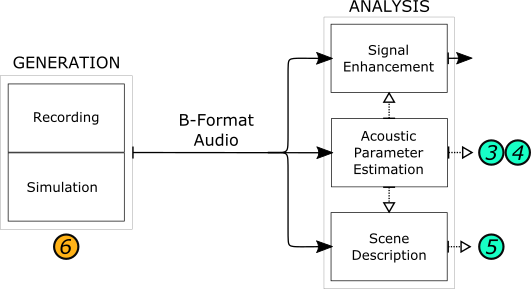
\includegraphics[width=\textwidth]{Figures/Introduction/SCHEME1_NUMBERS.png}
%  \caption{General scheme of the B-Format audio generation and analysis framework, including the thesis contributions in form of Chapter numbers.}
%  \label{fig:scheme1_numbers2}
%\end{figure}




\section{Future Work}

This thesis has tackled several research problems associated with the analysis of ambisonic recordings, making use primarily of the parametric sound field modelling analysis.
The presented techniques improve existing state-of-the-art methodologies, or present novel approaches for known research problems, which in turn bring new research questions. \\

%Chapter~\ref{chap:rt60} presents a novel methodology for the blind estimation of reverberation time from ambisonic audio. The method is based on two main steps: first, dereverberation using a multichannel auto-recursive model (MAR), and second, estimation of the  filter from reverberant and dereverberated signals. The actual reverberation time value is estimated from the energy decay of the estimated filter. 
%
%The proposed system is the first attempt in the literature to address the blind reverberation time estimation problem specifically for ambisonic signals. Compared with a state-of-the-art monophonic estimator, our method is able to improve in all the standard evaluation metrics under consideration.

A novel blind reverberation time estimation method for first-order ambisonic recordings is introduced in Chapter~\ref{chap:rt60}.
Among others, the method could be straightforwardly extended to higher order ambisonic signals, which might still improve the reported results due to the availability of many more audio channels. 
Moreover, the usage of online MAR methods would enable the possibility of analyzing sound scenes with moving sources; the statistical time-invariance property of late reverberation supports this hypothesis.
Finally, it is important to mention that the proposed method is resource-intensive. An analysis of the trade-off between computation time and evaluation performance, mostly dependent on the estimation filter length, remains to be done.  
\newpage
Given the current interest in the field of augmented reality, new related research topics emerge. One of them, which has been recently baptized as \textit{acoustic matching} \cite{su2020acoustic}, deals with the analysis of acoustic properties of real enclosures, with the aim of later introduction of virtual elements whose reverberation would match real conditions. 
The application of our method to the acoustic matching problem is straightforward: given an ambisonic recording with a target reverberation, estimate its reverberation time and synthesize a reverberant tail with the target energy decay; early reflections might be generated by various methods, including physical models or perceptually motivated approaches. 
We can foresee a growing interest on the topic in the near future; our contribution might help to establish the foundation of a new family of methods. \\


%In Chapter~\ref{chap:coherence}, we have characterised the response of tetrahedral microphones to isotropic noise field, which is one of the most used models for diffuse sound. Furthermore, the capabilities of a spherical loudspeaker array with respect to the reconstruction of diffuse sound fields using ambisonics are also tested. 
Regarding the diffuse field characterization performed in Chapter~\ref{chap:coherence}, an immediate extension of the work would include the study of different spherical microphone array geometries, from the ones that are commercially available.
The usage of different models of diffuse fields, specially extending to the anisotropic case \cite{alary2019assessing}, might also constitute an interesting research continuation direction. 
Both cases could be also applied to the experiment of diffuse sound field reconstruction using loudspeaker arrays. \\

%in Future work in this direction might include the characterisation of different spherical microphone array geometries, and different types of diffuse field models. Additionally, the experiment on loudspeaker array diffuse field reconstruction could be easily extended, with the aim of including more . \\


%Chapter~\ref{chap:seld2019} describes an algorithm for sound event localization and detection (SELD), developed in the context of the DCASE 2020 challenge. The method estimates the localization and temporal activity of the sound events based on a particle filter that tracks event trajectories obtained from the parametric analysis of the ambisonic sound field. Each event is assigned to a sound class by a machine learning classifier that uses low- and mid- level audio features. Results on the cross-validation development set show a significant performance increase in most evaluation metrics, compared with a state-of-the-art deep learning baseline. This result shows that our approach, which is substantially different to the baseline and the majority of state-of-the-art methods, represents an alternative in specific situations with low-complexity or small database constraints. 

The wide scope of the SELD problem, as described in Chapter~\ref{chap:seld2019}, allows for a wide range of possibilities regarding a potential follow-up of the proposed method.
For instance, one of the major problems of our algorithm is the inaccurate parametric estimation when two events are simultaneously active. Although it is a known problem in the literature \cite{epain2016spherical} , a successful solution in the given context remains still to be explored.
\newpage
Another source of potential improvements is the refinement of the particle filter applied to this specific task. A deeper understanding of control theory, as well as collaborations with experts on the field, might bring a noticeable improvement on the overall system performance.

The performance of the event classifier might be also further analyzed. Although in this case we opted for a classical feature-based machine learning approach, different methods and architectures could be compared, including more modern deep-learning approaches.\\

%Finally, the thesis contributions to more practical aspects are presented in Chapter~\ref{chap:data}. Those contributions comprise two software libraries written in Python: one of them focused on spherical microphone array and acoustic simulation, and another one implementing the SOFA standard, which has also been revised and modified for allowing the representation of ambisonic data. Finally, a software for the procedural creation of annotated reverberant ambisonic datasets has ben also presented. 

Finally, we discuss briefly on the practical contributions described in  Chapter~\ref{chap:data}.
Apart from the straightforward task of software maintenance, the engagement of the research community with the usage and eventual contribution of the libraries would represent a desired situation in the near future.
Moreover, the proposed file format convention is being currently discussed by the \textit{Standardisation Committee on AES-69 Standard}, which can be considered a great achievement of the original proposal. 
The results of the discussion might lead to the addition of a modified version of our proposal into version 2 of the \textit{AES-69 Standard}. 


In the medium term, the application at commercial level of some of the methods  described in this thesis would be a highly desirable outcome of our research. Such application would probably imply a re-implementation at the software level, intended for compatibility with the workflows and formats used in the VR/AR content production industry. 


\newpage
\section{List of Contributions}

In the following list we show the main scientific contributions, as main author, related to this dissertation:

\begin{itemize}

	\item Peer-reviewed journal articles
	
	\textbf{"Analysis of spherical isotropic noise fields with an A-Format tetrahedral microphone"}.
	\underline{A. P\'erez-L\'opez} and N. Stefanakis.
	\textit{The Journal of the Acoustical Society of America 146.4 (2019): EL329-EL334.}

	\item Peer-reviewed conference articles

	\textbf{"Blind reverberation time estimation from ambisonic recordings"}.
	\underline{A. P\'erez-L\'opez}, A. Politis and E. G\'omez.
	Submitted to \textit{IEEE 22nd International Workshop on Multimedia Signal Processing, 2020.}\\

	\textbf{"PAPAFIL: a low complexity sound event localization and detection method with parametric particle filtering and gradient boosting".}
	\underline{A. P\'erez-L\'opez} and R. Iba�ez-Usach.
	Submitted to \textit{Detection and Classification of Acoustic Scenes and Events 2020 Workshop (DCASE2020)}.\\
	
	\textbf{"A hybrid parametric-deep learning approach for sound event localization and detection".}
	\underline{A. P\'erez-L\'opez}, E. Fonseca and X. Serra.
	In \textit{Proceedings of the Detection and Classification of Acoustic Scenes and Events 2019 Workshop (DCASE2019)}.
	
	\textbf{"Ambiscaper: A tool for automatic generation and annotation of reverberant ambisonics sound scenes".}\\
	\underline{A. P\'erez-L\'opez}.
	In \textit{Proceedings of the 16th International Workshop on Acoustic Signal Enhancement (IWAENC). IEEE, 2018.}
	
	
	\item Conference engineering briefs


	\textbf{"Ambisonics directional room impulse response as a new convention of the spatially oriented format for acoustics".}
	\underline{A. P\'erez-L\'opez} and J. De Muynke.
	In \textit{Proceedings of the 144th Audio Engineering Society Convention. Audio Engineering Society, 2018.}\\
	
	\textbf{"pysofaconventions, a Python API for SOFA".}
	\underline{A. P\'erez-L\'opez}.
	In \textit{Proceedings of the 148th Audio Engineering Society Convention. Audio Engineering Society, 2020.}\\
	
	\textbf{"A Python library for multichannel acoustic signal processing".}
	\underline{A. P\'erez-L\'opez} and A. Politis.
	In \textit{Proceedings of the 148th Audio Engineering Society Convention. Audio Engineering Society, 2020.}\\
	
\end{itemize}


Moreover, although not strictly aligned with the research direction of this thesis, the author has supervised the following publication:\\

	 \textbf{"Sound event localization and detection based on CRNN using dense rectangular filters and channel rotation data augmentation".}
	F. Ronchini, D. Arteaga and \underline{A. P\'erez-L\'opez}.
	Submitted to \textit{Detection and Classification of Acoustic Scenes and Events 2020 Workshop (DCASE2020)}.\\


\newpage
\section{List of Software Resources}


As a result of the development of this thesis, the following open-source libraries and repositories have been produced. All of them are freely available through the author's GitHub page \cite{andresgithub} under open-source licenses. 


\begin{itemize}

	\item Software tools:

	
	\href{https://github.com/andresperezlopez/masp}{masp: Multichannel Acoustic Signal Processing library} 
		Tools for acoustic simulation and spherical array processing. \\
		 
	\href{https://github.com/andresperezlopez/pysofaconventions}{pysofaconventions} Implementation of the SOFA convention in Python.\\ 
	
	\href{https://github.com/andresperezlopez/AmbisonicsDRIR}{AmbisonicsDRIR}	 Ambisonic SOFA Convention proposal.\\

	\href{https://github.com/andresperezlopez/ambiscaper}{AmbiScaper} Tool for automatic generation of annotated ambisonic datasets.\\

	\item Method implementations: 

	\href{https://github.com/andresperezlopez/ambisonic_rt_estimation}{ambisonic\_rt\_estimation} Contains the code implementing the methods described in Chapter~\ref{chap:rt60}.\\
	
	\href{https://github.com/andresperezlopez/DCASE2020}{DCASE2020} Full code implementing the SELD algorithm from Chapter~\ref{chap:seld2019}.\\
	
	\href{https://github.com/andresperezlopez/DCASE2019_task3}{DCASE2019\_task3} 
		Implementation of the method submitted to DCASE2019 (not included in this thesis). \\


\end{itemize}



